%-------------------------
% Resume in Latex
% Author : Jake Gutierrez
% Based off of: https://github.com/sb2nov/resume
% License : MIT
%------------------------

\documentclass[letterpaper,11pt]{article}

\usepackage[T5]{fontenc} % Support Vietnamese characters with pdfLaTeX.
\usepackage{latexsym}
\usepackage[empty]{fullpage}
\usepackage{titlesec}
\usepackage{marvosym}
\usepackage[usenames,dvipsnames]{color}
\usepackage{verbatim}
\usepackage{enumitem}
\usepackage[hidelinks]{hyperref}
\usepackage{fancyhdr}
\usepackage[english]{babel}
\usepackage{tabularx}
\usepackage{graphicx}
\usepackage{fontawesome5}
\input{glyphtounicode}


%----------FONT OPTIONS----------
% sans-serif
% \usepackage[sfdefault]{FiraSans}
% \usepackage[sfdefault]{roboto}
% \usepackage[sfdefault]{noto-sans}
% \usepackage[default]{sourcesanspro}

% serif
% \usepackage{CormorantGaramond}
% \usepackage{charter}


\pagestyle{fancy}
\fancyhf{} % clear all header and footer fields
\fancyfoot{}
\renewcommand{\headrulewidth}{0pt}
\renewcommand{\footrulewidth}{0pt}

% Adjust margins
\addtolength{\oddsidemargin}{-0.5in}
\addtolength{\evensidemargin}{-0.5in}
\addtolength{\textwidth}{1in}
\addtolength{\topmargin}{-.5in}
\addtolength{\textheight}{1.0in}

\urlstyle{same}

\raggedbottom
\raggedright
\setlength{\tabcolsep}{0in}

% Sections formatting
\titleformat{\section}{
  \vspace{-4pt}\scshape\raggedright\large
}{}{0em}{}[\color{black}\titlerule \vspace{-5pt}]

% Ensure that generate pdf is machine readable/ATS parsable
\pdfgentounicode=1

%-------------------------
% Custom commands
\newcommand{\resumeItem}[1]{
  \item\small{
    {#1 \vspace{0pt}}
  }
}

\newcommand{\resumeSubheading}[4]{
  \vspace{-2pt}\item
    \begin{tabular*}{0.97\textwidth}[t]{l@{\extracolsep{\fill}}r}
      \textbf{#1} & #2 \\
      \textit{\small#3} & \textit{\small #4} \\
    \end{tabular*}\vspace{-7pt}
}

\newcommand{\resumeSubSubheading}[2]{
    \item
    \begin{tabular*}{0.97\textwidth}{l@{\extracolsep{\fill}}r}
      \textit{\small#1} & \textit{\small #2} \\
    \end{tabular*}\vspace{-7pt}
}

\newcommand{\resumeProjectHeading}[2]{
    \item
    \begin{tabular*}{0.97\textwidth}{l@{\extracolsep{\fill}}r}
      \small#1 & #2 \\
    \end{tabular*}\vspace{-7pt}
}

\newcommand{\resumeSubItem}[1]{\resumeItem{#1}\vspace{-4pt}}

\renewcommand\labelitemii{$\vcenter{\hbox{\tiny$\bullet$}}$}

% Match every content bullet list to Library74's existing spacing.
% Text remains \small through \resumeItem (10pt text, 12pt baseline).
\SetEnumitemKey{resumeBulletSpacing}{
  topsep=4.5pt plus 2pt minus 1pt,
  itemsep=2pt plus 1pt minus 1pt,
  parsep=2pt plus 1pt minus 1pt,
  partopsep=3pt plus 1pt minus 1pt
}

\newcommand{\resumeSubHeadingListStart}{\begin{itemize}[leftmargin=0.15in, label={}]}
\newcommand{\resumeSubHeadingListEnd}{\end{itemize}}
\newcommand{\resumeItemListStart}{\begin{itemize}[resumeBulletSpacing]}
\newcommand{\resumeItemListEnd}{\end{itemize}\vspace{-5pt}}

%-------------------------------------------
%%%%%%  RESUME STARTS HERE  %%%%%%%%%%%%%%%%%%%%%%%%%%%%


\begin{document}

%----------HEADING----------
\begin{center}
  \begin{minipage}[c]{0.82\textwidth}
    \centering
    \textbf{\Huge \scshape Võ Quang Thắng} \\ \vspace{1pt}
    \small \href{tel:+84399728845}{\faIcon{phone}\enspace 0399728845} $|$ \href{mailto:vqthang2004@gmail.com}{\faIcon{envelope}\enspace\underline{vqthang2004@gmail.com}} $|$
    \href{https://www.linkedin.com/in/th%E1%BA%AFng-quang-b8b794302}{\faIcon{linkedin}\enspace\underline{LinkedIn}} $|$
    \href{https://github.com/quangthangk4}{\faIcon{github}\enspace\underline{GitHub}} \\
    \small Fresher Java Backend Developer $|$ \faIcon{map-marker-alt}\enspace TP.HCM
  \end{minipage}\hfill
  \begin{minipage}[c]{0.14\textwidth}
    \raggedleft
    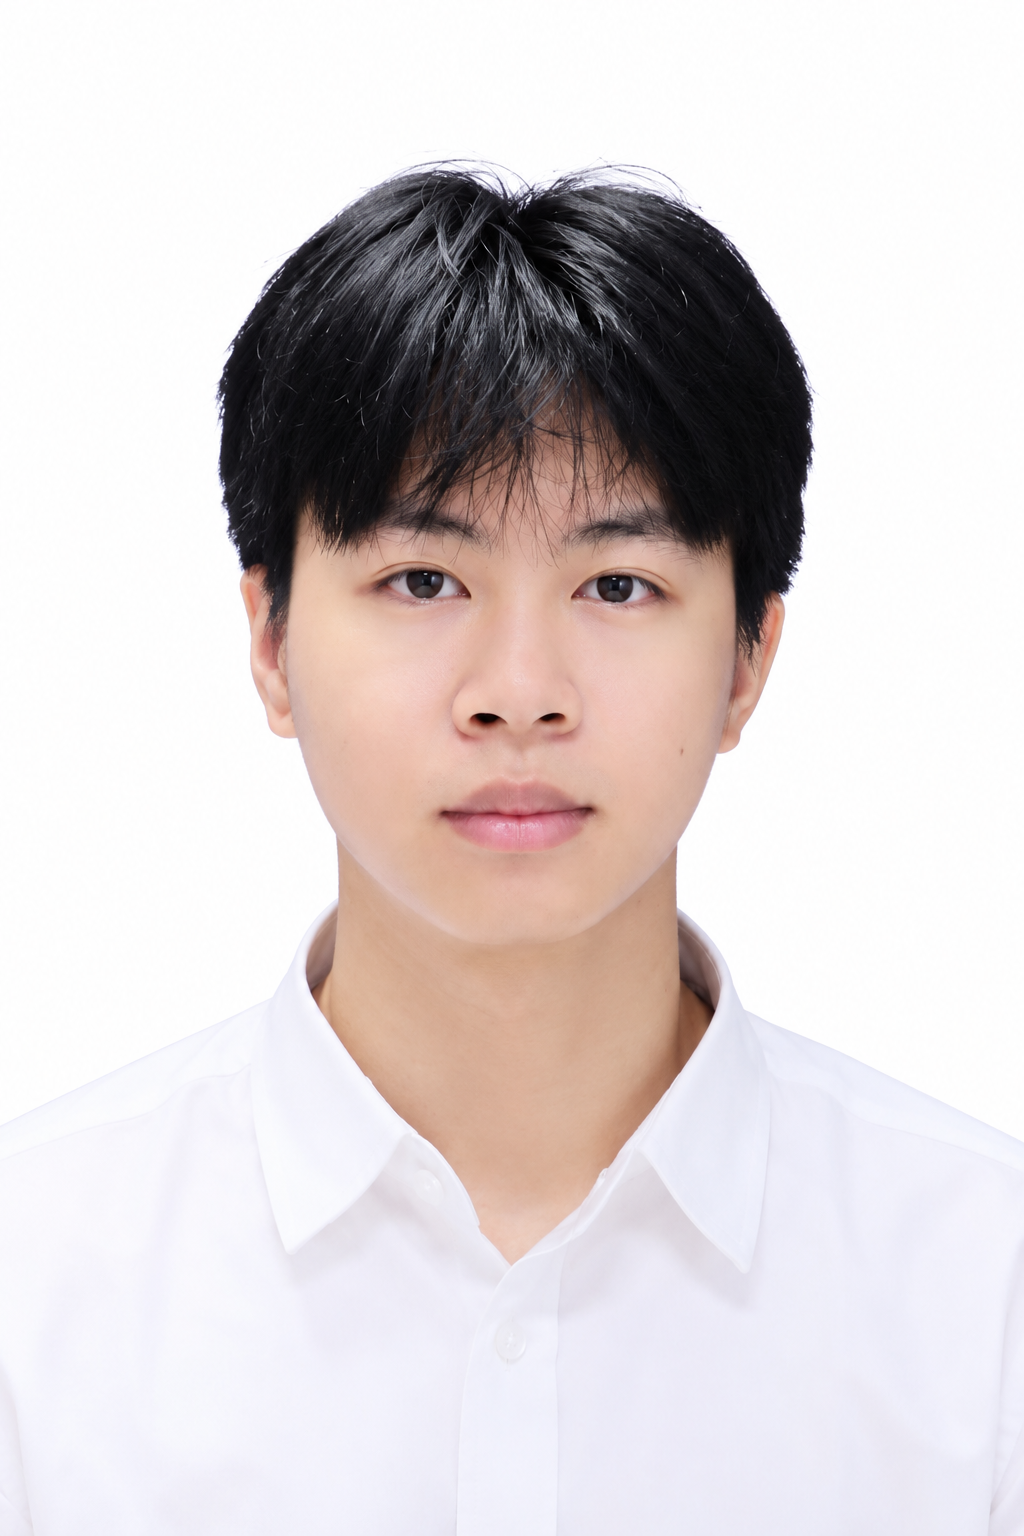
\includegraphics[width=22mm]{asset/anh_tot_nghiep.png}
  \end{minipage}
\end{center}


%-----------OBJECTIVE-----------
\section{Objective}
{\small Seeking a Java Backend Developer position to apply my knowledge of Java and Spring Boot in building reliable and scalable backend systems while continuously improving my technical skills.\par}


%-----------EDUCATION & CERTIFICATIONS-----------
\section{Education \& Certifications}
  \resumeSubHeadingListStart
    \resumeSubheading
      {Ho Chi Minh City University of Technology (HCMUT)}{TP.HCM, Vietnam}
      {Bachelor of Computer Science}{09/2022 -- 10/2026}
      \resumeItemListStart
        \resumeItem{\textbf{TOEIC Listening \& Reading: 705} (05/2026)}
        \resumeItem{\textbf{TOEIC Speaking \& Writing: 210} (09/2026; taken at HCMUT)}
      \resumeItemListEnd
  \resumeSubHeadingListEnd


%-----------EXPERIENCE-----------
\section{Experience}
  \resumeSubHeadingListStart

    \resumeSubheading
      {Java Backend Developer Intern}{04/2025 -- 10/2025}
      {Công ty TNHH Tư vấn và Phát triển Giáo dục InnEdu}{}
      \begin{itemize}[leftmargin=0.15in, label={}, topsep=3pt, itemsep=2pt, parsep=0pt]
        \item {\small\textbf{Learnmigo}}
          \begin{itemize}[resumeBulletSpacing, leftmargin=0.2in, label={\tiny$\bullet$}, topsep=1pt, itemsep=1pt, parsep=0pt, partopsep=0pt]
            \resumeItem{Developed user management features and bulk-imported questions from Excel files.}
            \resumeItem{Developed a gamification system featuring user rankings and level-based feature unlocking.}
            \resumeItem{Fixed backend bugs and resolved frontend integration issues based on code review feedback.}
          \end{itemize}
        \item {\small\textbf{Resource Marketplace}}
          \begin{itemize}[resumeBulletSpacing, leftmargin=0.2in, label={\tiny$\bullet$}, topsep=1pt, itemsep=1pt, parsep=0pt, partopsep=0pt]
            \resumeItem{Implemented authentication and role-based access control using JWT and Spring Security.}
            \resumeItem{Implemented direct-to-storage file uploads using S3-compatible presigned URLs.}
          \end{itemize}
      \end{itemize}\vspace{-5pt}

  \resumeSubHeadingListEnd


%-----------PROJECTS-----------
\section{Projects}
    \resumeSubHeadingListStart
      \resumeSubheading
          {\small Library74 --- AI-powered Library Management System}{10/2025 -- 05/2026}
          {Graduation Project: 9.2/10}
          {\href{https://github.com/quangthangk4/LMS}{\faIcon{github}\enspace\underline{GitHub}} $|$ \href{https://library74.uk}{\faIcon{external-link-alt}\enspace\underline{Demo}} $|$ \href{https://drive.google.com/file/d/1YmcTygbzFZaRTrhOL5eMPB9bT1LfSry7/view?usp=sharing}{\faIcon{play-circle}\enspace\underline{Video}} $|$ \href{https://drive.google.com/file/d/1waUzJBUj230gCykyno_ewdixoRylv9dE/view?usp=sharing}{\faIcon{file-pdf}\enspace\underline{Report}}}
          \resumeItemListStart
            \resumeItem{\textbf{System Architecture:} Designed a Spring Boot modular monolith with domain-oriented Maven modules, JWT/OAuth2, RBAC, and Kafka-based asynchronous notifications.}
            \resumeItem{\textbf{AI Chatbot:} Built a Gemini-powered chatbot with RAG, function calling for authenticated data retrieval, and Redis-based conversation memory.}
            \resumeItem{\textbf{AI Integration \& Semantic Search:} Built a FastAPI PDF processing pipeline for text extraction, chunking, and Gemini-based metadata extraction; implemented SBERT embeddings and pgvector search, achieving 87.5\% Recall@5 and 0.907 nDCG@5.}
            \resumeItem{\textbf{Recommendation System:} Implemented personalized book recommendations using content-based filtering, ALS, and trending-based fallback.}
            \resumeItem{\textbf{Database \& Reliability:} Designed PostgreSQL schemas, managed Flyway migrations, implemented row-level locking, and cached recommendation rankings in Redis.}
            \resumeItem{\textbf{Testing \& Deployment:} Tested business logic and transaction rollback using JUnit, Mockito, and Testcontainers; deployed to a Linux VPS using Docker Compose and GitHub Actions CI/CD, with database backups and health checks.}
          \resumeItemListEnd
    \resumeSubHeadingListEnd


%-----------PROGRAMMING SKILLS-----------
\section{Technical Skills}
 \begin{itemize}[leftmargin=0.15in, label={}]
    \small{\item{
     \textbf{Languages}{: Java, SQL} \\
     \textbf{Backend}{: Spring Boot, Spring Security, Spring Data JPA, REST APIs, JWT, OAuth2} \\
     \textbf{Data \& Messaging}{: PostgreSQL, Redis, Apache Kafka, Flyway} \\
     \textbf{AI \& Machine Learning}{: Gemini API, RAG, SBERT, Semantic Search} \\
     \textbf{Testing}{: JUnit 5, Mockito, Testcontainers, Gatling} \\
     \textbf{Tools}{: Git, Maven, Docker, Linux, Nginx, GitHub Actions}
    }}
 \end{itemize}


%-------------------------------------------
\end{document}
